	\section*{Exercice 3 (5 points)}
	

	\subsection*{1. Justifier que la superficie de l’enclos, en m$^2$, est donnée en fonction de $x$ par $g(x) = 4xe^{-0,5x}$ pour $x$ dans l’intervalle $[0; 5]$.}
	
	Pour $x \in [0; 5]$, on a $OA = x$ et $OC = f(x) = 4e^{-0,5x}$.\\ On a donc
	\[
	A(OABC) = x \times f(x) = 4xe^{-0,5x}
	\]
	
	\subsection*{2. La fonction $g$ est dérivable sur $[0; 5]$. Montrer que, pour tout réel $x$ de l’intervalle $[0; 5]$, on a $g'(x) = (4 - 2x)e^{-0,5x}$.}
	
	Pour $x \in [0; 5]$, on a
	\[
	g'(x) = 4e^{-0,5x} + 4xe^{-0,5x} \times (-0,5) = 4e^{-0,5x} - 2xe^{-0,5x} = (4 - 2x)e^{-0,5x}
	\]
	
	\subsection*{3. En déduire le tableau de variations de la fonction $g$ sur $[0; 5]$.}
	
	On sait que quel que soit le réel $a$, $e^a > 0$ ; le signe de $g'(x)$ est donc celui de $4 - 2x$.	
 $4 - 2x > 0 \iff 4 > 2x \iff x < 2 $\\
	Sur l’intervalle $[0; 2]$, la dérivée est positive, donc la fonction $g$ est croissante de $g(0) = 0$ à $g(2) = 8e^{-1} \approx 2,943$.
 $g(2) = 8e^{-1}$ et $g(5) = 20e^{-2,5} \approx 1,642$.

	
	Le tableau de variation est donc :
\begin{center}
		\begin{tikzpicture}[double distance=2pt]
		\tkzTabInit{$x$/1,$f'(x)$/1,$f(x)$/2}{$0$,$2$, $5$}
		\tkzTabLine{,+,z, -}
		\tkzTabVar{-/$0$,+/ $8\e^{-1}$ /, -/$20\e^{-2,5}$}
	\end{tikzpicture}
\end{center}

	
	\subsection*{4. Où doit-on placer le point $A$ sur $[OD]$ pour obtenir une superficie d’enclos maximale ? Donner la superficie maximale possible en arrondissant le résultat au dm$^2$.}
	
	D’après la question précédente l’enclos aura une surface maximale pour $x = 2$ et on a vu que $g(2) \approx 2,943$, soit 2,94 m$^2$ au dm$^2$ près.
	
